% CVPR 2027, articolo principale (8 pagine di corpo + riferimenti), versione per la revisione (anonima).
% Kit autori in paper/cvpr_kit/ (quello di CVPR 2026, SEGNAPOSTO finche' non esce il kit 2027).
% Supplementary separato: supp_cvpr.tex (riferimenti incrociati con xr-hyper, prefisso S-; compilare prima main,
% poi supp, poi di nuovo main: containers/texbuild/scripts/compile_paper.sbatch lo fa).
% La bozza precedente (15 pagine di corpo) e' main_cvpr_draft.tex, invariata.
%
% Regole di questo file (12 ottobre 2026):
% - ogni numero ha un commento "% fonte: file:riga" (righe dei CSV: 1 = intestazione); le tabelle in tables/ sono
%   generate da figs/scripts/make_tables.py e portano la fonte per ogni cella;
% - "\todo{matrice}" = dipende dalla matrice unificata (aau/runs/evidence/full_matrix/, in corso);
%   "\todo{run}" = concorrente in corso (ULRSSM, Hybrid FM, Gromov-Wasserstein, feature su render);
%   "\todo{Ava}" = conferma su Ava-256 (protocollo confermativo in preparazione: NESSUN numero Ava qui);
% - tutto cio' che e' post hoc e' dichiarato come tale nel testo; i risultati sfavorevoli restano (qui o nel supp).
\documentclass[10pt,twocolumn,letterpaper]{article}

\usepackage[review]{cvpr_kit/cvpr}      % versione per la revisione
% \usepackage{cvpr_kit/cvpr}            % versione finale (camera-ready)

\usepackage[utf8]{inputenc}
\usepackage[T1]{fontenc}
\usepackage{url}
\usepackage{booktabs}
\usepackage{amsfonts}
\usepackage{amsmath}
\usepackage{microtype}
\usepackage{graphicx}
\usepackage{xcolor}
\usepackage{tikz}
\usetikzlibrary{positioning,arrows.meta,calc}
\newcommand{\todo}[1]{\textcolor{red}{\textbf{TODO:} #1}}
\newcommand{\ci}[3]{#1\,{\tiny[#2,\,#3]}}
\newcommand{\pd}[3]{$#1$~[$#2$, $#3$]}  % differenza appaiata con IC nel testo
\newif\ifshowcommits\showcommitsfalse
\newcommand{\commit}[1]{\ifshowcommits\texttt{#1}\else\textit{anon.}\fi}

\definecolor{cvprblue}{rgb}{0.21,0.49,0.74}
\usepackage{xr-hyper}
\usepackage[pagebackref,breaklinks,colorlinks,allcolors=cvprblue]{hyperref}
\externaldocument[S-]{supp_cvpr}

\def\paperID{*****} % TODO: ID dell'articolo assegnato da OpenReview
\def\confName{CVPR}
\def\confYear{2027} % il kit e' quello 2026 (segnaposto)

\title{When Alignment Hurts: Removing More Than Pose Erases Identity in 3D Face Comparison}
% Sottotitolo proposto il 12 ottobre: la rigida (la posa) aiuta, togliere di piu' (la taglia per mesh, una
% deformazione non rigida per coppia) peggiora l'ordinamento per forma. Alternativa: "...: Pose-Only Alignment Keeps
% Identity, Scale and Pairwise Deformation Erase It".

\author{%
  Anonymous Authors \\
  Anonymous Institution \\
  \texttt{anonymous@example.com}
}

\begin{document}

\twocolumn[{%
\renewcommand\twocolumn[1][]{#1}%
\maketitle
\vspace{-1.2em}
\begin{center}
  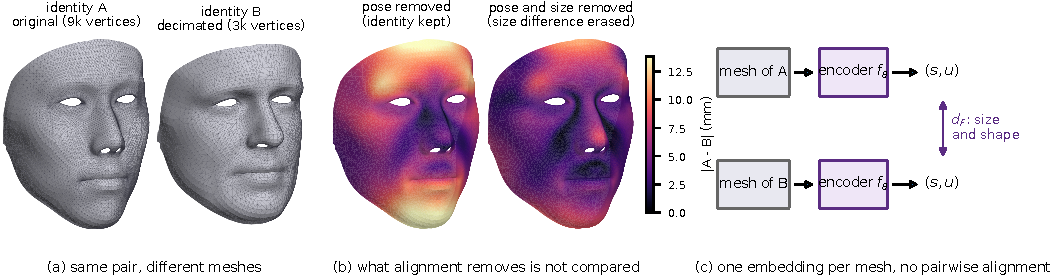
\includegraphics[width=\textwidth]{figs/fig_teaser.pdf}
  \captionof{figure}{\textbf{What an alignment removes is no longer compared.} (a) Two synthetic identities of an
  openly licensed morphable model (GNM Head), stored with different discretizations. (b) Per-vertex difference in dense
  correspondence after removing pose with one rigid fit per identity (left) and after also normalizing size (right): the
  size difference, an identity trait, disappears from the comparison. (c) Our metric embeds each mesh once and compares
  embeddings that keep size and shape, with no pairwise alignment. Illustration only; all numbers are in
  Secs.~\ref{sec:alignment}--\ref{sec:fewshot}.}
  \label{fig:teaser}
\end{center}
\vspace{0.6em}
}]

\begin{abstract}
% fonti: tables/tab_scale.tex (punti con FR, righe di spearman_e2.csv e baselines_mm/spearman.csv indicate li');
% 0.749 [0.673, 0.806]: aau/runs/evidence/baselines_param/spearman_e2.csv:10; 0.642: spearman_e2.csv:2;
% pari a ICP in mm -0.001 [-0.055, +0.055]: aau/runs/evidence/trainer_v3/factorized_paired.csv:3;
% pari alle composizioni taglia stimata + registrazione senza scala: factorized_paired.csv:112-113;
% FaceScape, fit con il modello nel ciclo: aau/runs/evidence/baselines_param/paired_e2.csv:3676, 3682, 3767-3768;
% FaMoS: factorized_paired.csv:4830; D5: aau/runs/evidence/diagnostics/results_d5.md, "Lettura preregistrata".
Comparing 3D faces that come from different templates and resolutions is usually done by aligning each pair of meshes and then measuring a distance. We ask whether such distances rank identities correctly, and make the reference explicit: a \emph{form} reference that keeps facial size and removes only pose, with one robust rigid fit per identity, and a \emph{shape} reference that also removes size. On held-out face generators and real scans, always across different discretizations, removing pose helps, but removing more than pose does not: normalizing size, or deforming one mesh onto the other, ranks identities by form below a rigid alignment in millimetres in all four families we test. Representations that encode each mesh alone in a common space (a template registration, a 3DMM fit, a learned embedding) do not show this systematic loss, although none of them beats rigid alignment everywhere. Size matters: where it varies, size alone ranks form better than any registration pipeline. We propose a registration-free encoder whose embedding factorizes into a log-size and a shape code, combined by the size-and-shape decomposition of geometric morphometrics. On HIFI3D, without boundary crops, its form distance reaches a Spearman correlation of 0.749 [0.673, 0.806] with a post-hoc calibration, above rigid alignment, template registration and 3DMM fits, but only level with compositions of an estimated size and a scale-free registration; the pre-registered, uncalibrated distance is level with rigid alignment. Where size barely varies, a 3DMM fitted with the model in the loop ranks shape and form better; the advantage does not replicate on 15 real subjects; boundary crops break the encoder. Its metric head adapts to a new generator with about 50 labelled identities. All protocols were written before the results they govern; every amendment is reported.
\end{abstract}

% =================================================================================================================
\section{Introduction}
\label{sec:intro}

Single-image and multi-view 3D face reconstruction methods now produce meshes with many different templates, topologies and resolutions~\cite{3ddfav2,deca,emoca,mica,deep3d,synergynet}. To compare such meshes, evaluation protocols align each predicted mesh to the ground truth and measure a geometric error~\cite{now,REALY,feng2018evaluation,facescape,ramon2021h3d}. The alignment usually removes more than pose. NoW~\cite{now} and the benchmark of Feng et al.~\cite{feng2018evaluation} fit a similarity transform from landmarks, so each pair gets its own scale; DECA and EMOCA report NoW in this setting~\cite{deca,emoca}; H3DS~\cite{ramon2021h3d} calls a library registration whose default also estimates a scale; REALY~\cite{REALY} estimates a scale from keypoints, refines each facial region with its own rigid fit, and uses a non-rigid registration of the ground truth to establish correspondences. FaceScape~\cite{zhu2023facescape} avoids ICP and fits only a depth offset (or, in its lab setting, one depth-scale factor).
% fonte: protocolli letti nel codice ufficiale, /tmp/.../scratchpad/protocolli_benchmark.md (ricognizione del 12
% ottobre 2026: now_evaluation scan2mesh_computations.py:126,:53; fg2018 compute_vertices_to_mesh_distances.py:25-28;
% h3ds numeric.py:44-46,61-62 con il default scale=True di trimesh; REALY utils/gICP.py:47, rICP.py:82, eval.py:78-103;
% facescape evaluator.py:96-131, 424-435). Non e' un file del repo: va copiato in paper/ o in literature/ se il PI lo vuole
% citabile come fonte. TODO verificare H3DS eseguendolo (la scala per default e' dedotta dalla lettura di trimesh).

We are not the first to see that these degrees of freedom matter. MICA~\cite{mica} showed that optimizing the scale favours methods that are not metrical and introduced a metrical NoW protocol with a purely rigid alignment; REALY~\cite{REALY} showed that the choice of alignment reference changes the results; Sariyanidi et al.~\cite{10448898} and M3DFB~\cite{fg2025} meta-evaluated error estimates on synthetic data. What is missing is a test of what the alignment does to \emph{identity}: if a distance is used to compare reconstructions, it must at least order pairs of different people correctly, and to check that one needs a reference distance that does not discard identity itself.

We therefore treat 3D face distances as a metric meta-evaluation problem with two explicit references (Sec.~\ref{sec:references}). The \emph{form} reference (FR) keeps size, an identity trait, and removes pose with one robust rigid fit per identity, never per pair; the \emph{shape} reference (SR) also removes size. Against them we measure, on face generators never used in training and on real scans, and always between meshes with different discretizations, how well each distance ranks pairs of identities. Our findings are:

\noindent\textbf{(A) Removing more than pose erases identity.} A rigid alignment in millimetres ranks form better than an unaligned Chamfer distance, but normalizing size or deforming one mesh onto the other ranks it worse, in all four families (Sec.~\ref{sec:alignment}). We are not aware of a published measurement of this effect for pairwise non-rigid alignment; we report it as our observation, with paired intervals still pending (\todo{matrice}). Encoding each mesh alone in a common space does not show this systematic loss.

\noindent\textbf{(B) Size matters.} Where size varies, size alone ranks form better than every registration pipeline, and a distance that keeps both size and shape is needed (Sec.~\ref{sec:size}).

\noindent\textbf{(C) A registration-free encoder.} We propose an encoder that embeds each mesh once, in millimetres, into a log-size and a shape code combined by the size-and-shape decomposition~\cite{kendall1984shape,dryden2016statistical} (Sec.~\ref{sec:method}). Trained only on synthetic samples of three morphable models, it ranks HIFI3D form better than rigid alignment, template registration and 3DMM fits, with a post-hoc calibration; it is level with simple compositions of an estimated size and a scale-free registration; it loses to a 3DMM fitted with the model in the loop where size barely varies; it does not replicate on 15 real subjects; it is not robust to boundary crops (Secs.~\ref{sec:results} and~\ref{sec:limitations}). Its metric head adapts to a new generator with about 50 labelled identities (Sec.~\ref{sec:fewshot}).

All analyses follow protocols written before the results they govern; post-hoc amendments are marked as such in the text and listed with their hashes in Supp.~\ref{S-sec:protocols}. Results that do not favour our method stay in the paper or in the supplementary.

% =================================================================================================================
\section{Related Work}
\label{sec:related}

\paragraph{Evaluating 3D face reconstruction.} Most evaluations compute nearest-neighbour or scan-to-mesh distances after rigid registration via ICP~\cite{besl1992icp,deng2019accurate,gecer2019ganfit,genova18,prnet,feng2018evaluation,sariyanidi20}, after landmark alignment~\cite{liu2018disentangling,zhu2020beyond}, or after non-rigid registration~\cite{amberg2007nicp,ferrari2021sparse,booth20163d,gilani2017dense}. The standard benchmarks differ mainly in the degrees of freedom they remove per pair (Sec.~\ref{sec:intro}). MICA~\cite{mica} is the closest prior work on scale: it measured how much a fitted scale lowers the error of a non-metrical prediction. We extend the question from scale to non-rigid alignment and from error magnitude to identity ranking, and we separate per-pair from per-mesh processing.

\paragraph{Metric meta-evaluation.} Synthetic data with known correspondence allows estimated errors to be compared with a reference~\cite{10448898,fg2025}; perceptual and learned similarity has been studied for 2D faces and textured shapes~\cite{huang2026alignface,luan2025tge} and for errors computed after registration~\cite{shilova2026curvature}. We use real scans as well as synthetic generators, and an explicit size-preserving reference.

\paragraph{Distances without correspondence.} Currents~\cite{vaillant2005surface} and varifolds compare surfaces as measures without a parameterization; both are special cases of the oriented-varifold kernel metrics of Kaltenmark et al.~\cite{kaltenmark2017general}, and Besnier et al.~\cite{besnier2023meshinvariant} used varifold losses to make 3D generative models invariant to the mesh. Gromov--Wasserstein distances~\cite{memoli2011gw} compare metric-measure spaces without alignment. Learned spectral matching (ULRSSM~\cite{cao2023ulrssm}, Hybrid Functional Maps~\cite{bastian2024hybrid}) builds dense correspondences across discretizations on the DiffusionNet backbone~\cite{diffusionet} we also use. Learned point-cloud distances~\cite{urbach2020dpdist} and image-space perceptual metrics~\cite{lpips,fu2023dreamsim,oquab2023dinov2,radford2021clip} are further candidates. We evaluate a varifold baseline here and are running Gromov--Wasserstein, retrained ULRSSM and Hybrid Functional Maps, and render-based perceptual features (\todo{run}). We found no public weights usable on our meshes for 3D face recognition networks (Led3D~\cite{mu2019led3d} works on depth images, and its weights could not be confirmed) or for scan-to-mesh face registration networks (Shape My Face~\cite{bahri2021smf} has not released code or weights), and DPDist~\cite{urbach2020dpdist} has no released weights; we did not find feed-forward regressors from scans to 3DMM parameters with public weights, so we compare with 3DMM fits by optimization (Sec.~\ref{sec:competitors}).
% fonte: /tmp/.../scratchpad/competitor_shortlist.md, voci [V]: Led3D (repo MIT, immagini di profondita', pesi non
% confermati), SMF ("Code coming soon", nessun peso), DPDist ("pre-trained models will be available soon"). Regressori
% scan -> 3DMM: esito negativo marcato [S + V parziale] nella shortlist: formulato come "non abbiamo trovato".
% Currents e varifold come casi particolari: abstract di Kaltenmark et al. 2017 (openaccess.thecvf.com, letto il 12 ott).

\paragraph{Size and shape.} Geometric morphometrics separates the size of a configuration (its centroid size) from its shape~\cite{kendall1984shape,dryden2016statistical} and uses resistant fits~\cite{siegel1982resistant}; we borrow both to define the references and the factorized head.

% =================================================================================================================
\section{Meta-Evaluating 3D Face Distances}
\label{sec:protocol}

\subsection{Form and shape references}
\label{sec:references}
A candidate distance $D(X_i,X_j)$ between two observed meshes is judged by the Spearman correlation, over pairs of different identities, between $D$ and a reference distance between the identities. The reference needs correspondence, so it is computed on 1{,}478 points of a face region covered by every domain, in millimetres, with area weights.
% fonte: aau/runs/evidence/e8/summary.md (regione unificata, 1478 vertici); aau/runs/evidence/e12/protocol.md
Each identity $i$ is rigidly fitted \emph{once} to a fixed mean face with a resistant estimator, giving a configuration $a_i$, its centroid size $S_i$ and its unit-size pre-shape $z_i$; no transformation depends on the pair. FR is the area-weighted RMS distance between $a_i$ and $a_j$, SR the same distance between $z_i$ and $z_j$. Up to a small centroid term they obey the size-and-shape decomposition
\begin{equation}
d_{\mathrm{FR}}^2(i,j)\approx(S_i-S_j)^2+S_iS_j\,d_{\mathrm{SR}}^2(i,j),
\label{eq:size_shape}
\end{equation}
so FR mixes a size term and a shape term whose relative weight depends on how much size varies in a population. FR is our primary reference for metric data, SR the reference for shape alone. An earlier version of this work normalized each mesh by its own maximum coordinate, which removes size; Supp.~\ref{S-sec:legacy} reports those results.

\subsection{Domains, discretizations and statistics}
\label{sec:domains}
\textbf{Held-out generators and real scans.} Our encoder is trained only on samples of three morphable models (Sec.~\ref{sec:method}). We test on identities sampled from three other published models, never used in training: HIFI3D~\cite{bao2021hifi3d} (100 identities, primary), the FaceScape bilinear model~\cite{facescape} (100, our development set: it entered model selection) and FaceVerse~\cite{wang2022faceverse} (100, with expressions; a neutral view in the supplementary), and on the real scans of the 15 FaMoS test subjects~\cite{bolkart2023tempeh}. The three generators are synthetic; only FaMoS is real, and its intervals are wide. HIFI3D is not a clean test either: it was never used for training, but it entered two model-selection decisions and motivated a post-hoc calibration (Sec.~\ref{sec:method}).
% fonte: aau/zs3dmm/zs_identities.py (identita' campionate N(0,1) dai modelli), aau/runs/evidence/diagnostics/results_d3.md
% r. 3 ("campioni di 3DMM non visti dai bracci, non dati reali; reale e' solo FaMoS"); selezione: factorized_results.md
% ("Regola dual", emendamento 4 sez. 5) e trainer_v3/ablations/k_ablation/results.md (k_eig su HIFI3D, FaceScape, FaceVerse).

\textbf{Discretizations.} Each identity is stored as six meshes: the original, a smoothed and decimated remesh, a strong decimation (down8k), an upsampling (up60k), a noisy copy and a boundary crop. The primary rows pair meshes of different identities \emph{and} different discretizations without the crop (20 ordered pairs of discretizations); crops are analysed separately (Sec.~\ref{sec:limitations}).

\textbf{Statistics.} We report Spearman correlations with 95\% subject-level bootstrap intervals (1{,}000 replicates; subjects are resampled and their pairs rebuilt). Comparisons between methods are paired differences on the same rows and replicates; within a domain all rows of Tab.~\ref{tab:main} share one mask and one set of replicates. No correction for multiple comparisons is applied; comparisons are descriptive unless a pre-registered rule says otherwise.

\subsection{Distances compared}
\label{sec:competitors}
\textbf{Pairwise.} Chamfer distance between centred meshes; rigid ICP~\cite{besl1992icp} + Chamfer in millimetres; the same after normalizing each mesh to a common centroid size (``size-normalized''); pairwise non-rigid ICP~\cite{amberg2007nicp} in millimetres and size-normalized. \textbf{Per mesh.} Non-rigid ICP of each mesh to a common template; a varifold distance~\cite{kaltenmark2017general} in millimetres; size alone, estimated from the mesh or taken from the reference (an oracle control). \textbf{3DMM fits.} GNM Head~\cite{ploumpis2026gnmhead} (Apache-2.0; also one of our training generators) and FLAME 2023 Open~\cite{li2017flame} (CC~BY~4.0; never seen in training) are fitted to every mesh and compared through their identity coefficients or their identity meshes, read under FR and under SR. The pre-registered fit has a median surface error of 1.0--1.6\,mm; a post-hoc variant with the model in the loop lowers it to 0.29--0.56\,mm, and a post-hoc ``size + shape'' composition combines its size and shape like our Eq.~\eqref{eq:factorized}.
% fonte: aau/runs/evidence/baselines_param/results.md:61-62 (errore di superficie); PROTOCOL.md (preregistrato,
% sez. 7: letture _fr con FR, _sr con SR, coefficienti con entrambe); emendamenti 1-2 (post hoc).
For each fit we report the reading the protocol declared for each reference (identity mesh under FR in the FR column, under SR in the SR column; coefficients under both), not the best reading per cell; all readings are in Supp.~\ref{S-sec:tables}.

% =================================================================================================================
\section{A Registration-Free Size-and-Shape Encoder}
\label{sec:method}

\begin{figure*}[t]
  \centering
  \resizebox{0.92\textwidth}{!}{% Fig. 2: schema del metodo (TikZ, vettoriale). Incluso da main_cvpr.tex con % Fig. 2: schema del metodo (TikZ, vettoriale). Incluso da main_cvpr.tex con % Fig. 2: schema del metodo (TikZ, vettoriale). Incluso da main_cvpr.tex con \input{figs/fig_method}.
% Nessun numero di risultato: solo le scelte di architettura dichiarate nel testo (Sect. sec:method).
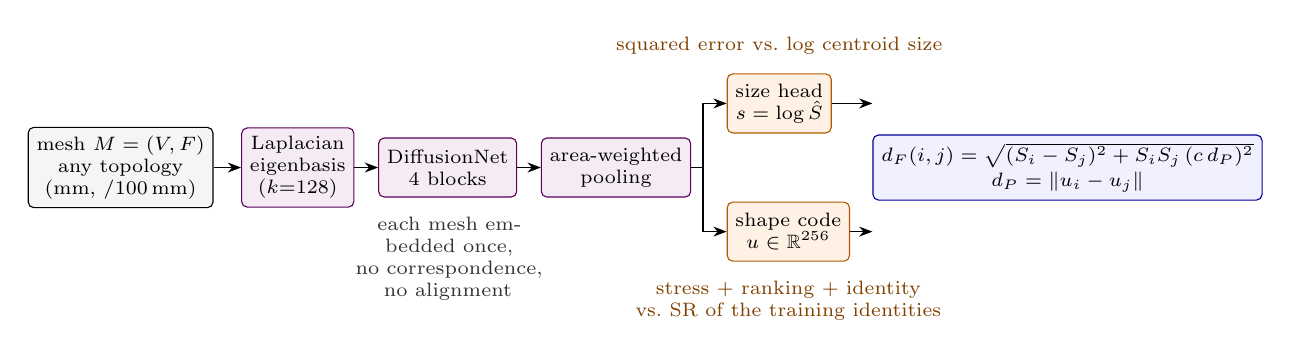
\begin{tikzpicture}[
  font=\scriptsize, >=Stealth,
  box/.style={draw, rounded corners=2pt, align=center, inner sep=3pt, minimum height=0.75cm},
  enc/.style={box, fill=violet!8, draw=violet!70!black},
  dat/.style={box, fill=gray!8},
  head/.style={box, fill=orange!10, draw=orange!70!black},
  dist/.style={box, fill=blue!6, draw=blue!60!black}]
  \node[dat] (m) {mesh $M=(V,F)$\\any topology\\(mm, $/100$\,mm)};
  \node[enc, right=0.35cm of m] (op) {Laplacian\\eigenbasis\\($k{=}128$)};
  \node[enc, right=0.3cm of op] (dn) {DiffusionNet\\4 blocks};
  \node[enc, right=0.3cm of dn] (pool) {area-weighted\\pooling};
  \node[head, above right=0.05cm and 0.45cm of pool] (s) {size head\\$s=\log \hat S$};
  \node[head, below right=0.05cm and 0.45cm of pool] (u) {shape code\\$u\in\mathbb R^{256}$};
  \draw[->] (m) -- (op); \draw[->] (op) -- (dn); \draw[->] (dn) -- (pool);
  \draw[->] (pool.east) -- ++(0.15,0) |- (s.west);
  \draw[->] (pool.east) -- ++(0.15,0) |- (u.west);
  \node[dist, right=0.4cm of $(s.east)!0.5!(u.east)$] (d)
    {$d_F(i,j)=\sqrt{(S_i-S_j)^2+S_iS_j\,(c\,d_P)^2}$\\[1pt] $d_P=\|u_i-u_j\|$};
  \draw[->] (s.east) -- (d.west |- s.east);
  \draw[->] (u.east) -- (d.west |- u.east);
  \node[below=0.12cm of u, align=center, text=orange!50!black] (lu) {stress + ranking + identity\\vs.\ SR of the training identities};
  \node[above=0.12cm of s, align=center, text=orange!50!black] (ls) {squared error vs.\ log centroid size};
  \node[below=0.12cm of dn, align=center, text=gray!40!black, text width=3.2cm]
    {each mesh embedded once,\\no correspondence, no alignment};
\end{tikzpicture}
.
% Nessun numero di risultato: solo le scelte di architettura dichiarate nel testo (Sect. sec:method).
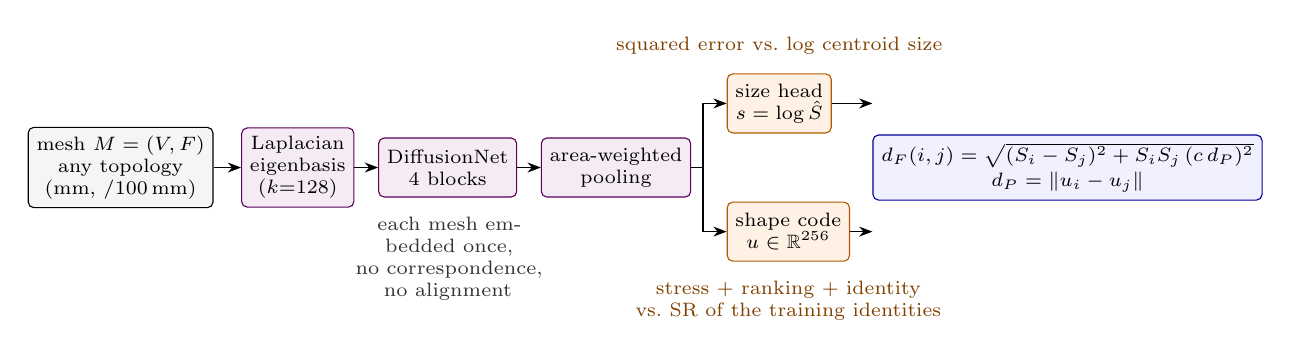
\begin{tikzpicture}[
  font=\scriptsize, >=Stealth,
  box/.style={draw, rounded corners=2pt, align=center, inner sep=3pt, minimum height=0.75cm},
  enc/.style={box, fill=violet!8, draw=violet!70!black},
  dat/.style={box, fill=gray!8},
  head/.style={box, fill=orange!10, draw=orange!70!black},
  dist/.style={box, fill=blue!6, draw=blue!60!black}]
  \node[dat] (m) {mesh $M=(V,F)$\\any topology\\(mm, $/100$\,mm)};
  \node[enc, right=0.35cm of m] (op) {Laplacian\\eigenbasis\\($k{=}128$)};
  \node[enc, right=0.3cm of op] (dn) {DiffusionNet\\4 blocks};
  \node[enc, right=0.3cm of dn] (pool) {area-weighted\\pooling};
  \node[head, above right=0.05cm and 0.45cm of pool] (s) {size head\\$s=\log \hat S$};
  \node[head, below right=0.05cm and 0.45cm of pool] (u) {shape code\\$u\in\mathbb R^{256}$};
  \draw[->] (m) -- (op); \draw[->] (op) -- (dn); \draw[->] (dn) -- (pool);
  \draw[->] (pool.east) -- ++(0.15,0) |- (s.west);
  \draw[->] (pool.east) -- ++(0.15,0) |- (u.west);
  \node[dist, right=0.4cm of $(s.east)!0.5!(u.east)$] (d)
    {$d_F(i,j)=\sqrt{(S_i-S_j)^2+S_iS_j\,(c\,d_P)^2}$\\[1pt] $d_P=\|u_i-u_j\|$};
  \draw[->] (s.east) -- (d.west |- s.east);
  \draw[->] (u.east) -- (d.west |- u.east);
  \node[below=0.12cm of u, align=center, text=orange!50!black] (lu) {stress + ranking + identity\\vs.\ SR of the training identities};
  \node[above=0.12cm of s, align=center, text=orange!50!black] (ls) {squared error vs.\ log centroid size};
  \node[below=0.12cm of dn, align=center, text=gray!40!black, text width=3.2cm]
    {each mesh embedded once,\\no correspondence, no alignment};
\end{tikzpicture}
.
% Nessun numero di risultato: solo le scelte di architettura dichiarate nel testo (Sect. sec:method).
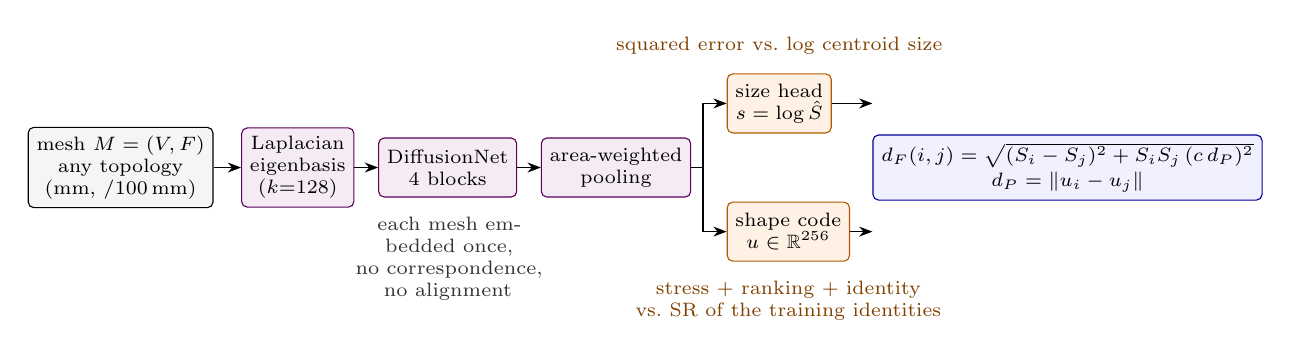
\begin{tikzpicture}[
  font=\scriptsize, >=Stealth,
  box/.style={draw, rounded corners=2pt, align=center, inner sep=3pt, minimum height=0.75cm},
  enc/.style={box, fill=violet!8, draw=violet!70!black},
  dat/.style={box, fill=gray!8},
  head/.style={box, fill=orange!10, draw=orange!70!black},
  dist/.style={box, fill=blue!6, draw=blue!60!black}]
  \node[dat] (m) {mesh $M=(V,F)$\\any topology\\(mm, $/100$\,mm)};
  \node[enc, right=0.35cm of m] (op) {Laplacian\\eigenbasis\\($k{=}128$)};
  \node[enc, right=0.3cm of op] (dn) {DiffusionNet\\4 blocks};
  \node[enc, right=0.3cm of dn] (pool) {area-weighted\\pooling};
  \node[head, above right=0.05cm and 0.45cm of pool] (s) {size head\\$s=\log \hat S$};
  \node[head, below right=0.05cm and 0.45cm of pool] (u) {shape code\\$u\in\mathbb R^{256}$};
  \draw[->] (m) -- (op); \draw[->] (op) -- (dn); \draw[->] (dn) -- (pool);
  \draw[->] (pool.east) -- ++(0.15,0) |- (s.west);
  \draw[->] (pool.east) -- ++(0.15,0) |- (u.west);
  \node[dist, right=0.4cm of $(s.east)!0.5!(u.east)$] (d)
    {$d_F(i,j)=\sqrt{(S_i-S_j)^2+S_iS_j\,(c\,d_P)^2}$\\[1pt] $d_P=\|u_i-u_j\|$};
  \draw[->] (s.east) -- (d.west |- s.east);
  \draw[->] (u.east) -- (d.west |- u.east);
  \node[below=0.12cm of u, align=center, text=orange!50!black] (lu) {stress + ranking + identity\\vs.\ SR of the training identities};
  \node[above=0.12cm of s, align=center, text=orange!50!black] (ls) {squared error vs.\ log centroid size};
  \node[below=0.12cm of dn, align=center, text=gray!40!black, text width=3.2cm]
    {each mesh embedded once,\\no correspondence, no alignment};
\end{tikzpicture}
}
  \caption{\textbf{Method.} Each mesh, in millimetres divided by one global constant, is embedded once by a DiffusionNet encoder with area-weighted pooling into a log-size $s$ and a shape code $u$; two meshes are compared by the size-and-shape distance $d_F$ (form) or by $d_P$ (shape). No correspondence, landmark or alignment is used at test time.}
  \label{fig:method}
\end{figure*}

\paragraph{Encoder.} A DiffusionNet~\cite{diffusionet} encoder (four blocks, width 128) receives vertex coordinates and precomputed surface operators (128 Laplacian eigenvectors on the mesh rescaled to unit area), and pools vertex features with area weights, so the embedding does not depend on the vertex count (Fig.~\ref{fig:method}). Coordinates are in millimetres in a common frame, divided by one global constant (100\,mm) instead of a per-mesh scale, so size stays visible. The encoder is not invariant to rotations by construction; robustness to small rigid motions comes from augmentation.
% fonte: aau/runs/evidence/trainer_v3/factorized.md, sez. 1 (ingresso globale /100 mm, pooling ad area, operatori areanorm k 128)

\paragraph{Factorized head.} The embedding is $[s,u]$: a shape code $u\in\mathbb R^{256}$, trained with a scale-normalized stress loss, a margin ranking loss and an identity-consistency term against the shape reference of the training identities, across their discretizations; and a scalar $s$, trained with a squared error against the log centroid size of the identity. Sizes are augmented by a log-uniform factor in $[0.8,1.25]$ applied to input and target. With $S_i=e^{s_i}$ and $d_P(i,j)=\|u_i-u_j\|$, the form distance follows Eq.~\eqref{eq:size_shape}:
\begin{equation}
d_F(i,j)=\sqrt{(S_i-S_j)^2+S_iS_j\,\big(c\,d_P(i,j)\big)^2}.
\label{eq:factorized}
\end{equation}
Loss terms and hyperparameters are in Supp.~\ref{S-sec:training}.

\paragraph{Calibration (post hoc).} The constant $c$ converts $d_P$ to the units of SR. We set it to the ratio of the median reference shape distance to the median $d_P$ over pairs of \emph{synthetic} held-out identities of the training generators (297{,}000 pairs), which gives $c=0.405$ for both seeds; no test identity enters its value. The calibration is a post-hoc amendment: it was added after the uncalibrated results were known, motivated in part by a check on HIFI3D, where the median shape term of the models was 8.6--15.7\,mm against 4.4\,mm in the reference. The pre-registered distance is $d_F$ with $c=1$; we report both.
% fonte: aau/runs/evidence/trainer_v3/factorized_results.md:11-12 (c = 0.405, 297000 coppie);
% aau/runs/evidence/trainer_v3/factorized_protocol_emendamento_4.md:1-12 (post hoc; 4.4 mm contro 8.6-15.7 mm, r. 9-10).

\paragraph{Training data.} Only synthetic samples of three morphable models: BFM, ICT-FaceKit~\cite{ict-facekit} and GNM Head (392, 4{,}557 and 844 training identities), each in all six discretizations including the crop; 21{,}096 steps, two seeds, EMA weights of the last checkpoint. GNM is therefore a prior our encoder has seen; FLAME 2023 Open is not.
% fonte: aau/runs/evidence/e1/summary.md:34 (cella C3F: BFM 392 + ICT 4.557 + GNM 844); factorized.md:89 (21.096 passi)

\paragraph{Few-shot adaptation.} On a new generator, the frozen embeddings can be re-weighted by a linear metric head $d=\|W u\|$, $W\in\mathbb R^{r\times 256}$, fitted with a stress loss on the shape reference of the source generators plus $k$ labelled identities of the target (Sec.~\ref{sec:fewshot}).
% fonte: aau/runs/evidence/diagnostics/PROTOCOL_D5.md, sez. 1 (testa i-e2, r in {32, 64}, lambda 1e-6, 7 sorgenti + k soggetti)

% =================================================================================================================
\section{Finding A: Removing More Than Pose Erases Identity}
\label{sec:alignment}

\begin{table}[t]
  \centering
  \scriptsize
  \caption{\textbf{Alignment scale.} Spearman correlation with the form reference (FR), cross-discretization pairs without crop, point estimates (95\% intervals in Supp.~\ref{S-sec:scale}). $\Delta$: paired difference against rigid ICP in millimetres on HIFI3D (unified matrix, pending). $^\dagger$Different row set (all 99{,}000 rows, no common mask).}
  \label{tab:scale}
  \setlength{\tabcolsep}{3pt}
  \resizebox{\linewidth}{!}{% GENERATO da paper/figs/scripts/make_tables.py: non modificare a mano, rigenerare.
% Ogni riga di tabella e' seguita da '% fonte:' con file:riga di ogni cella, nell'ordine.
% Scala dell'allineamento, GT FR, punti senza crop. Delta contro ICP rigido in mm: matrice unificata (aau/runs/evidence/full_matrix/paired.csv), NON ANCORA DISPONIBILE.
\begin{tabular}{lccccc}
\toprule
Distance & HIFI3D & FaceSc. & FaceV. & FaMoS & $\Delta$ HIFI3D \\
\midrule
\multicolumn{6}{l}{\emph{Pairwise}} \\
Chamfer, centred, no alignment$^\dagger$ & 0.411 & 0.211 & 0.281 & 0.623 & \todo{matrice} \\
% fonte: aau/runs/evidence/baselines_mm/spearman.csv:12, aau/runs/evidence/baselines_mm/spearman.csv:492, aau/runs/evidence/baselines_mm/spearman.csv:332, aau/runs/evidence/baselines_mm/spearman.csv:805, -
+ rigid ICP (pose) & 0.643 & 0.453 & 0.337 & 0.739 & ref. \\
% fonte: aau/runs/evidence/baselines_param/spearman_e2.csv:122, aau/runs/evidence/baselines_param/spearman_e2.csv:397, aau/runs/evidence/baselines_param/spearman_e2.csv:672, aau/runs/evidence/baselines_param/spearman_e2.csv:1146, -
+ size normalization & 0.358 & 0.416 & 0.290 & 0.601 & \todo{matrice} \\
% fonte: aau/runs/evidence/baselines_param/spearman_e2.csv:141, aau/runs/evidence/baselines_param/spearman_e2.csv:416, aau/runs/evidence/baselines_param/spearman_e2.csv:691, aau/runs/evidence/baselines_param/spearman_e2.csv:1161, -
+ non-rigid ICP$^\dagger$ & 0.495 & 0.374 & 0.201 & 0.719 & \todo{matrice} \\
% fonte: aau/runs/evidence/baselines_mm/spearman.csv:14, aau/runs/evidence/baselines_mm/spearman.csv:494, aau/runs/evidence/baselines_mm/spearman.csv:334, aau/runs/evidence/baselines_mm/spearman.csv:808, -
+ size norm. + non-rigid ICP & 0.376 & 0.346 & 0.212 & 0.584 & \todo{matrice} \\
% fonte: aau/runs/evidence/baselines_param/spearman_e2.csv:137, aau/runs/evidence/baselines_param/spearman_e2.csv:412, aau/runs/evidence/baselines_param/spearman_e2.csv:687, aau/runs/evidence/baselines_param/spearman_e2.csv:1157, -
\midrule
\multicolumn{6}{l}{\emph{Per mesh}} \\
NICP to a template (mm) & 0.614 & 0.542 & 0.212 & -- & \todo{matrice} \\
% fonte: aau/runs/evidence/baselines_param/spearman_e2.csv:126, aau/runs/evidence/baselines_param/spearman_e2.csv:401, aau/runs/evidence/baselines_param/spearman_e2.csv:676, -, -
FLAME fit (in the loop), identity mesh & 0.686 & 0.630 & 0.264 & 0.668 & \todo{matrice} \\
% fonte: aau/runs/evidence/baselines_param/spearman_e2.csv:237, aau/runs/evidence/baselines_param/spearman_e2.csv:512, aau/runs/evidence/baselines_param/spearman_e2.csv:787, aau/runs/evidence/baselines_param/spearman_e2.csv:1253, -
GNM fit (in the loop), identity mesh & 0.664 & 0.678 & 0.292 & 0.686 & \todo{matrice} \\
% fonte: aau/runs/evidence/baselines_param/spearman_e2.csv:213, aau/runs/evidence/baselines_param/spearman_e2.csv:488, aau/runs/evidence/baselines_param/spearman_e2.csv:763, aau/runs/evidence/baselines_param/spearman_e2.csv:1229, -
Ours, $d_F$ uncalibrated, seed 1 & 0.642 & 0.687 & 0.297 & 0.616 & \todo{matrice} \\
% fonte: aau/runs/evidence/baselines_param/spearman_e2.csv:2, aau/runs/evidence/baselines_param/spearman_e2.csv:277, aau/runs/evidence/baselines_param/spearman_e2.csv:552, aau/runs/evidence/baselines_param/spearman_e2.csv:1026, -
Ours, $d_F$ calibrated, seed 1 & 0.749 & 0.661 & 0.303 & 0.678 & \todo{matrice} \\
% fonte: aau/runs/evidence/baselines_param/spearman_e2.csv:10, aau/runs/evidence/baselines_param/spearman_e2.csv:285, aau/runs/evidence/baselines_param/spearman_e2.csv:560, aau/runs/evidence/baselines_param/spearman_e2.csv:1034, -
\bottomrule
\end{tabular}
}
\end{table}

Tab.~\ref{tab:scale} and Fig.~\ref{fig:scale} order the pairwise pipelines by the degrees of freedom they remove. A rigid alignment in millimetres, which removes pose, ranks form better than the centred, unaligned Chamfer distance on HIFI3D, FaceScape and FaceVerse (0.643 against 0.411, 0.453 against 0.211, 0.337 against 0.281) and on FaMoS (0.739 against 0.623). Removing more than pose lowers it in all four families: normalizing size gives 0.358, 0.416, 0.290 and 0.601; a pairwise non-rigid ICP in millimetres gives 0.495, 0.374, 0.201 and 0.719; both together 0.376, 0.346, 0.212 and 0.584. These are point estimates on two slightly different row sets; paired intervals come with the unified matrix (\todo{matrice}).
% fonte: tables/tab_scale.tex (righe: baselines_mm/spearman.csv:12,492,332,805 Chamfer; spearman_e2.csv:122,397,672,1146
% ICP mm; :141,416,691,1161 ICP cs; baselines_mm/spearman.csv:14,494,334,808 NICP mm; spearman_e2.csv:137,412,687,1157
% NICP cs). Delta appaiati ICP mm - Chamfer: non esistono (baselines_mm/paired.csv ha solo delta fra normalizzazioni).

\begin{figure}[t]
  \centering
  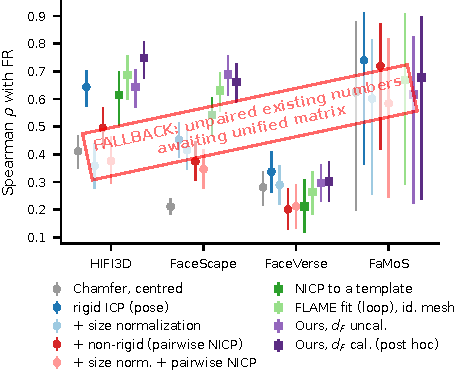
\includegraphics[width=\linewidth]{figs/fig_scale.pdf}
  \caption{\textbf{Alignment scale, by family} (FR). Circles: pairwise pipelines; squares: per-mesh representations. \todo{matrice: the current plot is a fallback with unpaired existing numbers; the final figure shows paired differences against rigid ICP in millimetres.}}
  \label{fig:scale}
\end{figure}

The loss is not a property of non-rigid registration as such. Registering each mesh non-rigidly to a \emph{common} template keeps the deformed template as its representation, and ranks form at 0.614, 0.542 and 0.212 on HIFI3D, FaceScape and FaceVerse: above pairwise non-rigid ICP on the first two and level on the third, though below rigid alignment on HIFI3D and FaceVerse. A 3DMM fit (identity mesh of FLAME with the model in the loop: 0.686, 0.630, 0.264, 0.668) and our encoder (0.642 uncalibrated, 0.749 calibrated on HIFI3D) also stay above pairwise non-rigid ICP on the three generators. None of the per-mesh representations is above rigid alignment everywhere: on FaceVerse and on FaMoS rigid ICP has the highest point estimate. Our reading is that an alignment chosen for each pair absorbs part of the very differences the reference measures (the size difference when it normalizes size, local shape differences when it deforms), while a representation fitted to each mesh alone cannot absorb a difference between two meshes it never sees together.
% fonte: tables/tab_scale.tex (NICP su template spearman_e2.csv:126,401,676; FLAME vB mesh FR :237,512,787,1253;
% nostri :2 e :10). FaMoS: NICP per coppia in mm 0.719 (baselines_mm/spearman.csv:808) sopra FLAME vB 0.668 e nostri
% 0.678 (spearman_e2.csv:1034): anche questo va detto (lo dice la frase "on FaMoS rigid ICP has the highest point
% estimate"; i due per-mesh stanno anche sotto NICP per coppia su FaMoS, in punto, 15 soggetti).

Under the shape reference the same degrees of freedom are \emph{required}, and the ladder changes accordingly: on HIFI3D, normalizing size raises rigid ICP from 0.365 to 0.580, and pairwise non-rigid ICP on size-normalized meshes reaches 0.595; on FaceScape and FaceVerse it stays below size-normalized rigid ICP (0.398 against 0.478, 0.235 against 0.306). An alignment hurts when it removes an invariance the reference does not have.
% fonte: tables/tab_main.tex, colonne SR (spearman_e2.csv:123,142,138 HIFI3D; 417,413 FaceScape; 692,688 FaceVerse)

\begin{figure}[t]
  \centering
  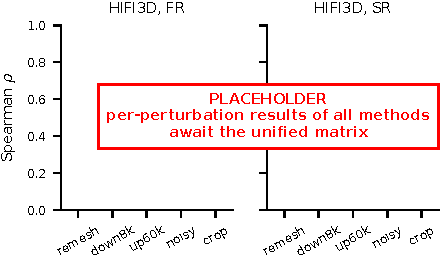
\includegraphics[width=\linewidth]{figs/fig_perturbation.pdf}
  \caption{\textbf{Robustness by discretization.} Spearman correlation on the pairs that involve each discretization, per method. \todo{matrice: placeholder; per-discretization results exist so far only for our encoder (Supp.~\ref{S-sec:topo}).}}
  \label{fig:perturbation}
\end{figure}

% =================================================================================================================
\section{Finding B: Size Matters, and Form Ranking on Held-Out Families}
\label{sec:results}

\subsection{Where size varies}
\label{sec:size}
Fig.~\ref{fig:size} explains why the families behave differently. On HIFI3D and FaMoS the centroid size of the evaluated identities varies with a coefficient of variation of 4.7\% and 4.4\%, and FR orders pairs quite differently from SR (Spearman 0.628 and 0.693 between the two references); on FaceScape and FaceVerse size varies by 1.6--1.8\% and FR orders pairs almost as SR does (0.888 and 0.954). Where size varies, size alone is a strong ranker of form: the oracle size reaches 0.737 on HIFI3D and 0.787 on FaMoS, and size estimated from the observed mesh 0.600 and 0.715, above every registration pipeline on HIFI3D (Tab.~\ref{tab:main}).
% fonte: aau/runs/evidence/baselines_param/controls_e2.json:62-63 (HIFI3D), :134-135 (FaMoS), :80-81 (FaceScape),
% :98-99 (FaceVerse); taglia oracolo spearman_e2.csv:134,1154; taglia stimata :130,1150.

\begin{figure}[t]
  \centering
  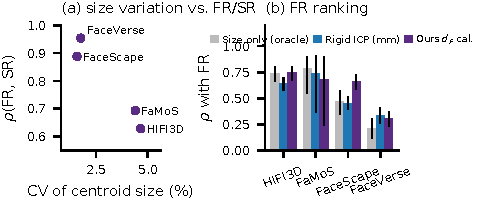
\includegraphics[width=\linewidth]{figs/fig_size.pdf}
  \caption{\textbf{Size.} (a) Coefficient of variation of centroid size and Spearman correlation between the FR and SR references, per family. (b) FR ranking by size alone (oracle), rigid ICP in millimetres and our calibrated $d_F$, with 95\% intervals.}
  \label{fig:size}
\end{figure}

\begin{table*}[t]
  \centering
  \scriptsize
  \caption{\textbf{Main results.} Spearman correlation ($\uparrow$) with the form (FR) and shape (SR) references on pairs of different identities and different discretizations, without crop; 95\% subject-level bootstrap intervals. Same rows and replicates for every method within a domain (HIFI3D 98{,}224 rows, FaceScape 88{,}725, FaceVerse 99{,}000, FaMoS 105). 3DMM fits: the declared reading for each reference, not the best per cell. ``Model in the loop'', ``size + shape'' and our calibration are post hoc; the pre-registered uncalibrated $d_F$ is shown next to it. FaceScape entered model selection; FaMoS has 15 real subjects. --: not a declared reading or not available. \todo{run}: competitor running.}
  \label{tab:main}
  \setlength{\tabcolsep}{2.2pt}
  \resizebox{\textwidth}{!}{% GENERATO da paper/figs/scripts/make_tables.py: non modificare a mano, rigenerare.
% Ogni riga di tabella e' seguita da '% fonte:' con file:riga di ogni cella, nell'ordine.
% Tabella principale: Spearman con FR e SR, coppie senza crop fra topologie diverse.
\begin{tabular}{lcccccccc}
\toprule
 & \multicolumn{2}{c}{\textbf{HIFI3D} (primary)} & \multicolumn{2}{c}{\textbf{FaceScape} (dev.)} & \multicolumn{2}{c}{\textbf{FaceVerse} (expr.)} & \multicolumn{2}{c}{\textbf{FaMoS} (15 subj.)} \\
\cmidrule(lr){2-3}\cmidrule(lr){4-5}\cmidrule(lr){6-7}\cmidrule(lr){8-9}
Method & FR & SR & FR & SR & FR & SR & FR & SR \\
\midrule
\multicolumn{9}{l}{\emph{Pairwise alignment (per pair of meshes)}} \\
Rigid ICP + Chamfer (mm) & \ci{0.643}{0.572}{0.702} & \ci{0.365}{0.280}{0.452} & \ci{0.453}{0.389}{0.514} & \ci{0.477}{0.414}{0.533} & \ci{0.337}{0.262}{0.410} & \ci{0.309}{0.234}{0.380} & \ci{0.739}{0.362}{0.914} & \ci{0.548}{0.185}{0.799} \\
% fonte: aau/runs/evidence/baselines_param/spearman_e2.csv:122, aau/runs/evidence/baselines_param/spearman_e2.csv:123, aau/runs/evidence/baselines_param/spearman_e2.csv:397, aau/runs/evidence/baselines_param/spearman_e2.csv:398, aau/runs/evidence/baselines_param/spearman_e2.csv:672, aau/runs/evidence/baselines_param/spearman_e2.csv:673, aau/runs/evidence/baselines_param/spearman_e2.csv:1146, aau/runs/evidence/baselines_param/spearman_e2.csv:1147
Size-normalized rigid ICP + Chamfer & \ci{0.358}{0.276}{0.438} & \ci{0.580}{0.529}{0.631} & \ci{0.416}{0.344}{0.485} & \ci{0.478}{0.412}{0.536} & \ci{0.290}{0.218}{0.358} & \ci{0.306}{0.233}{0.376} & \ci{0.601}{0.254}{0.815} & \ci{0.612}{0.306}{0.787} \\
% fonte: aau/runs/evidence/baselines_param/spearman_e2.csv:141, aau/runs/evidence/baselines_param/spearman_e2.csv:142, aau/runs/evidence/baselines_param/spearman_e2.csv:416, aau/runs/evidence/baselines_param/spearman_e2.csv:417, aau/runs/evidence/baselines_param/spearman_e2.csv:691, aau/runs/evidence/baselines_param/spearman_e2.csv:692, aau/runs/evidence/baselines_param/spearman_e2.csv:1161, aau/runs/evidence/baselines_param/spearman_e2.csv:1162
Size-normalized pairwise NICP & \ci{0.376}{0.296}{0.465} & \ci{0.595}{0.546}{0.648} & \ci{0.346}{0.276}{0.419} & \ci{0.398}{0.329}{0.464} & \ci{0.212}{0.131}{0.292} & \ci{0.235}{0.158}{0.310} & \ci{0.584}{0.243}{0.818} & \ci{0.775}{0.540}{0.860} \\
% fonte: aau/runs/evidence/baselines_param/spearman_e2.csv:137, aau/runs/evidence/baselines_param/spearman_e2.csv:138, aau/runs/evidence/baselines_param/spearman_e2.csv:412, aau/runs/evidence/baselines_param/spearman_e2.csv:413, aau/runs/evidence/baselines_param/spearman_e2.csv:687, aau/runs/evidence/baselines_param/spearman_e2.csv:688, aau/runs/evidence/baselines_param/spearman_e2.csv:1157, aau/runs/evidence/baselines_param/spearman_e2.csv:1158
Learned correspondence, ULRSSM (retrained), per pair & \todo{run} & \todo{run} & \todo{run} & \todo{run} & \todo{run} & \todo{run} & \todo{run} & \todo{run} \\
% fonte: -, -, -, -, -, -, -, -
Learned correspondence, Hybrid FM (retrained), per pair & \todo{run} & \todo{run} & \todo{run} & \todo{run} & \todo{run} & \todo{run} & \todo{run} & \todo{run} \\
% fonte: -, -, -, -, -, -, -, -
Gromov--Wasserstein (no correspondence) & \todo{run} & \todo{run} & \todo{run} & \todo{run} & \todo{run} & \todo{run} & \todo{run} & \todo{run} \\
% fonte: -, -, -, -, -, -, -, -
\midrule
\multicolumn{9}{l}{\emph{Per-mesh representation in a common space}} \\
NICP to a template (mm) & \ci{0.614}{0.506}{0.698} & \ci{0.083}{$-$0.018}{0.185} & \ci{0.542}{0.468}{0.605} & \ci{0.399}{0.320}{0.473} & \ci{0.212}{0.117}{0.308} & \ci{0.152}{0.058}{0.246} & -- & -- \\
% fonte: aau/runs/evidence/baselines_param/spearman_e2.csv:126, aau/runs/evidence/baselines_param/spearman_e2.csv:127, aau/runs/evidence/baselines_param/spearman_e2.csv:401, aau/runs/evidence/baselines_param/spearman_e2.csv:402, aau/runs/evidence/baselines_param/spearman_e2.csv:676, aau/runs/evidence/baselines_param/spearman_e2.csv:677, -, -
ULRSSM (retrained), via a template & \todo{run} & \todo{run} & \todo{run} & \todo{run} & \todo{run} & \todo{run} & \todo{run} & \todo{run} \\
% fonte: -, -, -, -, -, -, -, -
Hybrid FM (retrained), via a template & \todo{run} & \todo{run} & \todo{run} & \todo{run} & \todo{run} & \todo{run} & \todo{run} & \todo{run} \\
% fonte: -, -, -, -, -, -, -, -
Varifold (mm, unit mass) & \ci{0.494}{0.411}{0.567} & \ci{0.195}{0.126}{0.261} & \ci{0.264}{0.223}{0.299} & \ci{0.281}{0.246}{0.313} & \ci{0.260}{0.201}{0.313} & \ci{0.250}{0.193}{0.306} & \ci{0.688}{0.368}{0.902} & \ci{0.582}{0.170}{0.842} \\
% fonte: aau/runs/evidence/baselines_param/spearman_e2.csv:193, aau/runs/evidence/baselines_param/spearman_e2.csv:194, aau/runs/evidence/baselines_param/spearman_e2.csv:468, aau/runs/evidence/baselines_param/spearman_e2.csv:469, aau/runs/evidence/baselines_param/spearman_e2.csv:743, aau/runs/evidence/baselines_param/spearman_e2.csv:744, aau/runs/evidence/baselines_param/spearman_e2.csv:1209, aau/runs/evidence/baselines_param/spearman_e2.csv:1210
Size only, estimated from the mesh & \ci{0.600}{0.498}{0.690} & \ci{0.023}{$-$0.070}{0.111} & \ci{0.204}{0.136}{0.266} & \ci{0.094}{0.044}{0.144} & \ci{0.126}{0.037}{0.214} & \ci{0.080}{$-$0.002}{0.170} & \ci{0.715}{0.392}{0.885} & \ci{0.333}{$-$0.178}{0.687} \\
% fonte: aau/runs/evidence/baselines_param/spearman_e2.csv:130, aau/runs/evidence/baselines_param/spearman_e2.csv:131, aau/runs/evidence/baselines_param/spearman_e2.csv:405, aau/runs/evidence/baselines_param/spearman_e2.csv:406, aau/runs/evidence/baselines_param/spearman_e2.csv:680, aau/runs/evidence/baselines_param/spearman_e2.csv:681, aau/runs/evidence/baselines_param/spearman_e2.csv:1150, aau/runs/evidence/baselines_param/spearman_e2.csv:1151
Size only, oracle (control) & \ci{0.737}{0.657}{0.802} & \ci{0.074}{$-$0.025}{0.165} & \ci{0.464}{0.345}{0.571} & \ci{0.119}{0.022}{0.229} & \ci{0.209}{0.114}{0.307} & \ci{0.019}{$-$0.067}{0.106} & \ci{0.787}{0.546}{0.900} & \ci{0.213}{$-$0.232}{0.573} \\
% fonte: aau/runs/evidence/baselines_param/spearman_e2.csv:134, aau/runs/evidence/baselines_param/spearman_e2.csv:135, aau/runs/evidence/baselines_param/spearman_e2.csv:409, aau/runs/evidence/baselines_param/spearman_e2.csv:410, aau/runs/evidence/baselines_param/spearman_e2.csv:684, aau/runs/evidence/baselines_param/spearman_e2.csv:685, aau/runs/evidence/baselines_param/spearman_e2.csv:1154, aau/runs/evidence/baselines_param/spearman_e2.csv:1155
\midrule
\multicolumn{9}{l}{\emph{3DMM fit, pre-registered (GNM seen in training, FLAME not)}} \\
GNM, coefficients & \ci{0.619}{0.503}{0.710} & \ci{0.156}{0.047}{0.259} & \ci{0.488}{0.399}{0.561} & \ci{0.460}{0.376}{0.538} & \ci{0.220}{0.148}{0.286} & \ci{0.182}{0.104}{0.252} & \ci{0.624}{0.195}{0.883} & \ci{0.418}{$-$0.012}{0.772} \\
% fonte: aau/runs/evidence/baselines_param/spearman_e2.csv:169, aau/runs/evidence/baselines_param/spearman_e2.csv:170, aau/runs/evidence/baselines_param/spearman_e2.csv:444, aau/runs/evidence/baselines_param/spearman_e2.csv:445, aau/runs/evidence/baselines_param/spearman_e2.csv:719, aau/runs/evidence/baselines_param/spearman_e2.csv:720, aau/runs/evidence/baselines_param/spearman_e2.csv:1185, aau/runs/evidence/baselines_param/spearman_e2.csv:1186
GNM, identity mesh & \ci{0.608}{0.500}{0.693} & \ci{0.325}{0.205}{0.441} & \ci{0.465}{0.386}{0.538} & \ci{0.576}{0.483}{0.663} & \ci{0.227}{0.140}{0.311} & \ci{0.209}{0.129}{0.285} & \ci{0.586}{0.145}{0.859} & \ci{0.547}{0.188}{0.825} \\
% fonte: aau/runs/evidence/baselines_param/spearman_e2.csv:173, aau/runs/evidence/baselines_param/spearman_e2.csv:178, aau/runs/evidence/baselines_param/spearman_e2.csv:448, aau/runs/evidence/baselines_param/spearman_e2.csv:453, aau/runs/evidence/baselines_param/spearman_e2.csv:723, aau/runs/evidence/baselines_param/spearman_e2.csv:728, aau/runs/evidence/baselines_param/spearman_e2.csv:1189, aau/runs/evidence/baselines_param/spearman_e2.csv:1194
FLAME, coefficients & \ci{0.566}{0.444}{0.663} & \ci{0.159}{0.044}{0.268} & \ci{0.385}{0.299}{0.467} & \ci{0.396}{0.311}{0.476} & \ci{0.174}{0.109}{0.237} & \ci{0.152}{0.079}{0.218} & \ci{0.457}{0.064}{0.760} & \ci{0.390}{0.027}{0.713} \\
% fonte: aau/runs/evidence/baselines_param/spearman_e2.csv:181, aau/runs/evidence/baselines_param/spearman_e2.csv:182, aau/runs/evidence/baselines_param/spearman_e2.csv:456, aau/runs/evidence/baselines_param/spearman_e2.csv:457, aau/runs/evidence/baselines_param/spearman_e2.csv:731, aau/runs/evidence/baselines_param/spearman_e2.csv:732, aau/runs/evidence/baselines_param/spearman_e2.csv:1197, aau/runs/evidence/baselines_param/spearman_e2.csv:1198
FLAME, identity mesh & \ci{0.639}{0.532}{0.725} & \ci{0.287}{0.177}{0.398} & \ci{0.449}{0.366}{0.519} & \ci{0.469}{0.372}{0.561} & \ci{0.211}{0.137}{0.279} & \ci{0.155}{0.075}{0.228} & \ci{0.565}{0.134}{0.856} & \ci{0.412}{0.083}{0.748} \\
% fonte: aau/runs/evidence/baselines_param/spearman_e2.csv:185, aau/runs/evidence/baselines_param/spearman_e2.csv:190, aau/runs/evidence/baselines_param/spearman_e2.csv:460, aau/runs/evidence/baselines_param/spearman_e2.csv:465, aau/runs/evidence/baselines_param/spearman_e2.csv:735, aau/runs/evidence/baselines_param/spearman_e2.csv:740, aau/runs/evidence/baselines_param/spearman_e2.csv:1201, aau/runs/evidence/baselines_param/spearman_e2.csv:1206
\midrule
\multicolumn{9}{l}{\emph{3DMM fit, model in the loop (post hoc)}} \\
GNM, coefficients & \ci{0.550}{0.465}{0.628} & \ci{0.674}{0.610}{0.734} & \ci{0.565}{0.491}{0.636} & \ci{0.618}{0.548}{0.683} & \ci{0.226}{0.134}{0.299} & \ci{0.222}{0.124}{0.302} & \ci{0.606}{0.167}{0.836} & \ci{0.745}{0.418}{0.882} \\
% fonte: aau/runs/evidence/baselines_param/spearman_e2.csv:209, aau/runs/evidence/baselines_param/spearman_e2.csv:210, aau/runs/evidence/baselines_param/spearman_e2.csv:484, aau/runs/evidence/baselines_param/spearman_e2.csv:485, aau/runs/evidence/baselines_param/spearman_e2.csv:759, aau/runs/evidence/baselines_param/spearman_e2.csv:760, aau/runs/evidence/baselines_param/spearman_e2.csv:1225, aau/runs/evidence/baselines_param/spearman_e2.csv:1226
GNM, identity mesh & \ci{0.664}{0.570}{0.738} & \ci{0.607}{0.532}{0.679} & \ci{0.678}{0.615}{0.740} & \ci{0.854}{0.803}{0.894} & \ci{0.292}{0.205}{0.363} & \ci{0.327}{0.239}{0.402} & \ci{0.686}{0.307}{0.910} & \ci{0.766}{0.592}{0.880} \\
% fonte: aau/runs/evidence/baselines_param/spearman_e2.csv:213, aau/runs/evidence/baselines_param/spearman_e2.csv:218, aau/runs/evidence/baselines_param/spearman_e2.csv:488, aau/runs/evidence/baselines_param/spearman_e2.csv:493, aau/runs/evidence/baselines_param/spearman_e2.csv:763, aau/runs/evidence/baselines_param/spearman_e2.csv:768, aau/runs/evidence/baselines_param/spearman_e2.csv:1229, aau/runs/evidence/baselines_param/spearman_e2.csv:1234
GNM, size + shape & \ci{0.698}{0.612}{0.769} & -- & \ci{0.800}{0.741}{0.847} & -- & \ci{0.338}{0.255}{0.407} & -- & \ci{0.753}{0.393}{0.938} & -- \\
% fonte: aau/runs/evidence/baselines_param/spearman_e2.csv:245, -, aau/runs/evidence/baselines_param/spearman_e2.csv:520, -, aau/runs/evidence/baselines_param/spearman_e2.csv:795, -, aau/runs/evidence/baselines_param/spearman_e2.csv:1261, -
FLAME, coefficients & \ci{0.585}{0.503}{0.661} & \ci{0.585}{0.513}{0.652} & \ci{0.549}{0.467}{0.625} & \ci{0.592}{0.512}{0.663} & \ci{0.203}{0.121}{0.275} & \ci{0.193}{0.108}{0.271} & \ci{0.666}{0.269}{0.878} & \ci{0.714}{0.431}{0.877} \\
% fonte: aau/runs/evidence/baselines_param/spearman_e2.csv:233, aau/runs/evidence/baselines_param/spearman_e2.csv:234, aau/runs/evidence/baselines_param/spearman_e2.csv:508, aau/runs/evidence/baselines_param/spearman_e2.csv:509, aau/runs/evidence/baselines_param/spearman_e2.csv:783, aau/runs/evidence/baselines_param/spearman_e2.csv:784, aau/runs/evidence/baselines_param/spearman_e2.csv:1249, aau/runs/evidence/baselines_param/spearman_e2.csv:1250
FLAME, identity mesh & \ci{0.686}{0.597}{0.758} & \ci{0.597}{0.518}{0.673} & \ci{0.630}{0.555}{0.695} & \ci{0.820}{0.757}{0.870} & \ci{0.264}{0.183}{0.336} & \ci{0.293}{0.209}{0.368} & \ci{0.668}{0.292}{0.908} & \ci{0.791}{0.626}{0.889} \\
% fonte: aau/runs/evidence/baselines_param/spearman_e2.csv:237, aau/runs/evidence/baselines_param/spearman_e2.csv:242, aau/runs/evidence/baselines_param/spearman_e2.csv:512, aau/runs/evidence/baselines_param/spearman_e2.csv:517, aau/runs/evidence/baselines_param/spearman_e2.csv:787, aau/runs/evidence/baselines_param/spearman_e2.csv:792, aau/runs/evidence/baselines_param/spearman_e2.csv:1253, aau/runs/evidence/baselines_param/spearman_e2.csv:1258
FLAME, size + shape & \ci{0.712}{0.627}{0.781} & -- & \ci{0.731}{0.657}{0.794} & -- & \ci{0.302}{0.222}{0.372} & -- & \ci{0.708}{0.372}{0.923} & -- \\
% fonte: aau/runs/evidence/baselines_param/spearman_e2.csv:249, -, aau/runs/evidence/baselines_param/spearman_e2.csv:524, -, aau/runs/evidence/baselines_param/spearman_e2.csv:799, -, aau/runs/evidence/baselines_param/spearman_e2.csv:1265, -
\midrule
\multicolumn{9}{l}{\emph{Ours, registration-free (FR: $d_F$; SR: $d_P$)}} \\
$d_F$ calibrated (post hoc), seed 1 & \ci{0.749}{0.673}{0.806} & \ci{0.622}{0.550}{0.685} & \ci{0.661}{0.586}{0.727} & \ci{0.747}{0.677}{0.804} & \ci{0.303}{0.229}{0.374} & \ci{0.286}{0.215}{0.352} & \ci{0.678}{0.237}{0.897} & \ci{0.740}{0.548}{0.883} \\
% fonte: aau/runs/evidence/baselines_param/spearman_e2.csv:10, aau/runs/evidence/baselines_param/spearman_e2.csv:7, aau/runs/evidence/baselines_param/spearman_e2.csv:285, aau/runs/evidence/baselines_param/spearman_e2.csv:282, aau/runs/evidence/baselines_param/spearman_e2.csv:560, aau/runs/evidence/baselines_param/spearman_e2.csv:557, aau/runs/evidence/baselines_param/spearman_e2.csv:1034, aau/runs/evidence/baselines_param/spearman_e2.csv:1031
$d_F$ calibrated (post hoc), seed 2 & \ci{0.731}{0.657}{0.792} & \ci{0.613}{0.533}{0.688} & \ci{0.669}{0.597}{0.733} & \ci{0.753}{0.687}{0.813} & \ci{0.318}{0.249}{0.379} & \ci{0.313}{0.237}{0.377} & \ci{0.654}{0.214}{0.896} & \ci{0.728}{0.516}{0.869} \\
% fonte: aau/runs/evidence/baselines_param/spearman_e2.csv:26, aau/runs/evidence/baselines_param/spearman_e2.csv:23, aau/runs/evidence/baselines_param/spearman_e2.csv:301, aau/runs/evidence/baselines_param/spearman_e2.csv:298, aau/runs/evidence/baselines_param/spearman_e2.csv:576, aau/runs/evidence/baselines_param/spearman_e2.csv:573, aau/runs/evidence/baselines_param/spearman_e2.csv:1050, aau/runs/evidence/baselines_param/spearman_e2.csv:1047
$d_F$ uncalibrated (pre-registered), seed 1 & \ci{0.642}{0.570}{0.706} & -- & \ci{0.687}{0.612}{0.758} & -- & \ci{0.297}{0.229}{0.362} & -- & \ci{0.616}{0.222}{0.824} & -- \\
% fonte: aau/runs/evidence/baselines_param/spearman_e2.csv:2, -, aau/runs/evidence/baselines_param/spearman_e2.csv:277, -, aau/runs/evidence/baselines_param/spearman_e2.csv:552, -, aau/runs/evidence/baselines_param/spearman_e2.csv:1026, -
$d_F$ uncalibrated (pre-registered), seed 2 & \ci{0.631}{0.560}{0.697} & -- & \ci{0.698}{0.619}{0.770} & -- & \ci{0.317}{0.243}{0.383} & -- & \ci{0.612}{0.191}{0.831} & -- \\
% fonte: aau/runs/evidence/baselines_param/spearman_e2.csv:18, -, aau/runs/evidence/baselines_param/spearman_e2.csv:293, -, aau/runs/evidence/baselines_param/spearman_e2.csv:568, -, aau/runs/evidence/baselines_param/spearman_e2.csv:1042, -
\bottomrule
\end{tabular}
}
\end{table*}

\subsection{Form ranking on HIFI3D}
\label{sec:hifi}
Without crops, the calibrated form distance of our encoder (0.749 and 0.731 for the two seeds) is above rigid ICP + Chamfer in millimetres (\pd{+0.106}{+0.062}{+0.154}, \pd{+0.088}{+0.040}{+0.138}), non-rigid registration to a template (\pd{+0.134}{+0.085}{+0.188}, \pd{+0.117}{+0.066}{+0.171}) and the best declared reading of every 3DMM fit, including FLAME with the model in the loop (\pd{+0.063}{+0.023}{+0.101}, \pd{+0.045}{+0.004}{+0.085}); against the size-plus-shape compositions of the fits it is above GNM for one seed (\pd{+0.051}{+0.009}{+0.094}; \pd{+0.033}{-0.009}{+0.075}) and level with FLAME (\pd{+0.037}{-0.002}{+0.075}, \pd{+0.019}{-0.019}{+0.057}).
% fonte: aau/runs/evidence/trainer_v3/factorized_paired.csv:105,309 (ICP mm), :106,310 (NICP template);
% aau/runs/evidence/baselines_param/paired_e2.csv:244,692 (FLAME vB mesh FR), :246,694 (GNM vB composizione),
% :247,695 (FLAME vB composizione).

It is \emph{not} above everything that keeps size. It is level with the oracle size alone (\pd{+0.012}{-0.034}{+0.062}, \pd{-0.006}{-0.058}{+0.048}) and with two post-hoc compositions of an estimated size with a scale-free registration, calibrated like ours (with rigid ICP: \pd{+0.034}{-0.001}{+0.071}, \pd{+0.017}{-0.019}{+0.057}; with pairwise non-rigid ICP: \pd{+0.021}{-0.013}{+0.054}, \pd{+0.003}{-0.031}{+0.037}), and below the ceiling that combines the oracle size with size-normalized rigid ICP (\pd{-0.093}{-0.128}{-0.060}, \pd{-0.110}{-0.153}{-0.073}). A pre-registered criterion for ``form beyond size'' (partial correlation given the oracle size above rigid ICP and pairwise non-rigid ICP) is not met for either seed (partial Spearman 0.421 [0.325, 0.509] and 0.409 [0.316, 0.500], level with rigid ICP). The contribution on HIFI3D is therefore to combine an estimated size and a shape distance in one registration-free embedding, not to see more shape than registration does.
% fonte: factorized_paired.csv:108,312 (taglia oracolo), :112,316 (taglia stimata + ICP cs cal.), :113,317 (taglia
% stimata + NICP cs cal.), :111,315 (oracolo + ICP cs cal.); factorized_results.md:120-121 (parziale, "non soddisfatto");
% composizioni calibrate: factorized_protocol_emendamento_5.md (post hoc).

\textbf{Without the post-hoc calibration} the picture is weaker. The pre-registered distance scores 0.642 and 0.631: level with rigid ICP (\pd{-0.001}{-0.055}{+0.055}, \pd{-0.012}{-0.075}{+0.051}) and with the pre-registered FLAME fit (\pd{+0.003}{-0.073}{+0.081}, \pd{-0.008}{-0.088}{+0.074}), and below the oracle size (\pd{-0.094}{-0.160}{-0.022}, \pd{-0.105}{-0.177}{-0.026}), the FLAME size-plus-shape composition (\pd{-0.069}{-0.127}{-0.012}, \pd{-0.080}{-0.143}{-0.019}) and the two estimated-size compositions (\pd{-0.072}{-0.139}{-0.007}, \pd{-0.083}{-0.149}{-0.015} with rigid ICP; \pd{-0.086}{-0.148}{-0.024}, \pd{-0.097}{-0.159}{-0.034} with pairwise non-rigid ICP).
% fonte: spearman_e2.csv:2,18; factorized_paired.csv:3,207 (ICP mm), :6,210 (oracolo), :10,214 e :11,215 (composizioni
% con taglia stimata); paired_e2.csv:7,455 (FLAME preregistrato, mesh FR), :23,471 (FLAME vB composizione).

\textbf{Shape (SR).} Our $d_P$ (0.622, 0.613) is level with size-normalized pairwise non-rigid ICP (\pd{+0.027}{-0.029}{+0.083}, \pd{+0.018}{-0.046}{+0.082}) and with the 3DMM fits with the model in the loop (GNM coefficients \pd{-0.053}{-0.136}{+0.032}, \pd{-0.062}{-0.149}{+0.032}), without pairwise registration or fitting.
% fonte: factorized_paired.csv:71,275; paired_e2.csv:153,601

\subsection{Where size barely varies, and other families}
\label{sec:other}
On FaceScape, our development set, our distances lead the geometric pipelines (form: \pd{+0.207}{+0.160}{+0.257} over rigid ICP and \pd{+0.119}{+0.030}{+0.210} over template registration; shape: \pd{+0.349}{+0.291}{+0.401} over pairwise non-rigid ICP, seed 1), but a 3DMM fitted with the model in the loop is better. In shape, GNM reaches 0.854 and FLAME 0.820 against our 0.747 and 0.753 (GNM: \pd{-0.107}{-0.155}{-0.065}, \pd{-0.101}{-0.148}{-0.058}; FLAME: \pd{-0.074}{-0.129}{-0.022}, \pd{-0.067}{-0.120}{-0.014}). In form, we are level with the identity meshes read under FR (GNM \pd{-0.018}{-0.085}{+0.043}, FLAME \pd{+0.031}{-0.036}{+0.089}, seed 1) and below both size-plus-shape compositions (GNM \pd{-0.139}{-0.194}{-0.090}, \pd{-0.131}{-0.184}{-0.086}; FLAME \pd{-0.070}{-0.127}{-0.017}, \pd{-0.062}{-0.123}{-0.009}) and below the GNM identity mesh read under SR, a reading not declared for FR (\pd{-0.106}{-0.175}{-0.027}, \pd{-0.098}{-0.167}{-0.014}). Here the calibration hurts: it lowers FR from 0.687 and 0.698 (uncalibrated) to 0.661 and 0.669. Because size barely varies, whoever ranks shape best also ranks form best. This explanation is partial: FaceVerse has an equally narrow size distribution and there the fits do not win.
% fonte: factorized_paired.csv:3265 (ICP mm), :3266 (NICP template), :3231 (NICP per coppia cs); paired_e2.csv:3676,4124
% (GNM vB mesh SR, SR), :3682,4130 (FLAME vB mesh SR, SR), :3759 (GNM vB mesh FR), :3765 (FLAME vB mesh FR), :3767,4215
% e :3768,4216 (composizioni), :3760,4208 (GNM vB mesh SR letta con FR); spearman_e2.csv:277,293 (non calibrata) e
% :285,301 (calibrata); spearman_e2.csv:493,517 (0.854, 0.820).

On FaceVerse with expressions every method stays around 0.3 with FR and our calibrated distance is below rigid ICP in point estimate (\pd{-0.035}{-0.105}{+0.036}, \pd{-0.019}{-0.091}{+0.049}). On the 15 real FaMoS test subjects, the only real test set and the only one that never entered model selection, our calibrated distance (0.678, 0.654) is below rigid ICP + Chamfer in millimetres (0.739; \pd{-0.062}{-0.223}{+0.068}, \pd{-0.085}{-0.234}{+0.040}) and below the estimated size alone (0.715): the HIFI3D advantage does not reproduce even in sign, with intervals that do not resolve anything on 15 subjects.
% fonte: factorized_paired.csv:1688,1892 (FaceVerse), :4830,5002 (FaMoS, ICP mm), :4831,5003 (taglia stimata);
% spearman_e2.csv:1034,1050,1146,1150.

% =================================================================================================================
\section{Adapting to a New Generator}
\label{sec:fewshot}
Can a few labelled identities of a new generator correct the shape distance? A pre-registered diagnostic fits the linear head of Sec.~\ref{sec:method} on the source generators plus $k$ identities of each target (FaceScape, HIFI3D, FaceVerse, FLAME 2023; 10 draws per $k$), and evaluates on 100 other identities of the target. The pre-registered criterion, a mean gain over $d_P$ of at least $+0.05$ with SR at $k=20$ for both seeds, is \textbf{not met}: seed 1 gains \pd{+0.060}{+0.040}{+0.079}, seed 2 \pd{+0.039}{+0.016}{+0.064} (Fig.~\ref{fig:fewshot}). At $k=50$, the smallest $k$ of our grid at which both seeds pass, the gains are $+0.090$ and $+0.066$; the true threshold lies between 20 and 50, which we did not sample, and it holds for the mean of the four targets, not for each: on neutral FaceVerse seed 2 gains \pd{+0.018}{-0.050}{+0.088} at $k=50$. The gain from target identities is real from $k=5$ (over $k=0$: \pd{+0.009}{+0.005}{+0.013} and \pd{+0.009}{+0.005}{+0.012}), and FR never drops by more than 0.011 at $k=20$. The head configuration was fixed at the edge of its grid ($\lambda=10^{-6}$); a post-hoc refit at $\lambda=10^{-5}$ does not change the verdict at $k=20$ (\pd{+0.047}{+0.028}{+0.067} for seed 2). The targets are morphable-model samples, not real data.
% fonte: aau/runs/evidence/diagnostics/results_d5.md, "Lettura preregistrata" (r. 7-14) e tabella "media dei 4" (EQ, SR);
% d5_delta.csv (curva; righe nel file fig_fewshot.sources.txt); incremento su k = 0: results_d5.md, "Incremento su k = 0";
% FaceVerse neutra s2345 k = 50: tabella s2345 EQ SR; FR minimo -0.011: "Note del coder"; lambda 1e-5: note POST HOC
% (job 1070080 / 1070085). Protocollo PROTOCOL_D5.md (commit 484d638).

\begin{figure}[t]
  \centering
  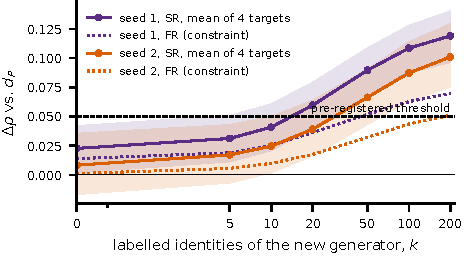
\includegraphics[width=\linewidth]{figs/fig_fewshot.pdf}
  \caption{\textbf{Few-shot adaptation.} Gain of the adapted head over $d_P$, mean of four target generators, as a function of the number $k$ of labelled target identities (pre-registered variant; band: 95\% interval with SR; dotted: FR). Dashed: pre-registered threshold at $k=20$.}
  \label{fig:fewshot}
\end{figure}

% =================================================================================================================
\section{Confirmation on Real Captures}
\label{sec:ava}
The only real test set above has 15 subjects. We are running a confirmatory test on Ava-256~\cite{martinez2024ava256} (CC~BY-NC~4.0), registered meshes of people never used in this project, with a protocol frozen before any method is evaluated on it: fixed calibration and evaluation splits, the same references, rows and statistics as above, and pre-declared comparisons with rigid ICP in millimetres, template registration and the 3DMM fits. \todo{Ava: protocollo confermativo congelato (hash), poi risultati; nessun numero prima.} Its capture pipeline shares the topology of Multiface, which entered our development, so its people are new but its acquisition domain is not independent.
% fonte: aau/ava256/README.md:3-7 (confermativo, nessuna valutazione prima del protocollo); PROTOCOL_CONFERMATIVO_bozza.md
% sez. 1-2 (bozza, voci [PI] aperte): nessun numero riportato qui per scelta.

% =================================================================================================================
\section{Limitations and Conclusion}
\label{sec:limitations}

\paragraph{Boundary crops.} Our encoder is not robust to boundary crops, although cropped meshes are in its training distribution. When pairs with a crop are added, its calibrated form distance on FaceScape falls from 0.661 and 0.669 to 0.370 and 0.351, about the level of rigid ICP on all pairs (0.381); on HIFI3D it falls to 0.709 and 0.661 (rigid ICP 0.556), and to 0.663 and 0.552 on the pairs that involve a crop. The 3DMM fits compare meshes on a region that excludes the boundary and barely move (GNM, shape, FaceScape: 0.854 without crop, 0.830 on crop pairs). A diagnostic shows that the crop shifts our predicted log size by about four times the between-subject spread on FaceScape; the mechanism is not identified (Supp.~\ref{S-sec:crop}).
% fonte: aau/runs/evidence/baselines_param/spearman_e3.csv:883,889 (FaceScape all_cross), :918 (ICP mm all_cross),
% :243,249 (HIFI3D all_cross), :278 (ICP mm HIFI3D all_cross), :403,409 (HIFI3D righe col crop), :1114 (GNM vB SR
% FaceScape righe col crop); spearman_e2.csv:493 (0.854 senza crop); spostamento di log S: baselines_param/results.md:151-154.

\paragraph{Size, shape and calibration.} Our HIFI3D advantage in form is not resolved against an oracle size or against estimated-size compositions, and rests on a post-hoc calibration that does not transfer exactly: the constant that would match medians is 0.503--0.507 on HIFI3D and 0.343--0.352 on FaceScape, against the 0.405 we use. Where size barely varies a 3DMM fit with the model in the loop ranks shape and form better, and on 15 real subjects the advantage does not replicate.
% fonte: aau/runs/evidence/trainer_v3/factorized_results.md:685-686

\paragraph{Scope.} Our references and all tests are on neutral or near-neutral shape; identities come mostly from morphable models, which inherit the demographics of their training populations (HIFI3D is an East-Asian model). We measure ranking of identity pairs, not the surface error of a reconstruction, and an encoder trained on faces could be misused for identification; we release recipes, seeds and openly licensed data only (Supp.~\ref{S-sec:data}). Per-mesh enrolment costs a few seconds on CPU, comparable to a 3DMM fit (Supp.~\ref{S-sec:cost}).

\paragraph{Conclusion.} Reconstruction benchmarks should declare their reference and separate one canonical fit per identity from pair-specific alignment: removing pose helps, removing size or deforming one mesh onto the other erases identity differences that the reference keeps. A registration-free size-and-shape embedding is one way to compare meshes without pairwise alignment; on our evidence it helps where size varies, and it is not yet a replacement for a well-fitted morphable model where shape alone matters.

{\small
\bibliographystyle{cvpr_kit/ieeenat_fullname}
\bibliography{references,refs_cvpr_add,refs_cvpr27}
}

\end{document}
